%
% Hauptdatei der Arbeit
%

\documentclass{scrartcl}

%Packages Definitionen
\usepackage[utf8x]{inputenc}
\usepackage[ngerman]{babel}


%------------------Anfang Nummerierung Anhang-----------------
\renewcommand\appendix{\par
\setcounter{section}{0}%
\setcounter{subsection}{0}%
\setcounter{figure}{0}%
\renewcommand\thesection{\Alph{section}} %
\renewcommand\thefigure{\Alph{section}.\arabic{figure}}}
%------------------Ende Nummerierung Anhang-----------------

%\input {deckblatt}


% Metadaten
\author{Sandro Ropelato, Christof Würmli}
\title{Fahrsimulator}

\begin{document}

%
% Titelseite der Projektarbeit
%

\begin{titlepage}
\vspace{4em}
\center

\Large{\textsf{Projektarbeit}}
\vspace{1em}

\Huge{\textsf{Fahrsimulator}}
\vspace{2em}
\\
\Large{
	\textsf{
		Sandro Ropelato (ropelsan)\\
		Christof Würmlil (wurmlchr)\\
		\vspace{2em}
		\today\\
		\vspace{2em}
		Studiengang: Systeminformatik SI\\
		Betreuender Dozent: Peter Früh (frup)
	}
}

\end{titlepage}

\section{Einleitung}
\subsection{Ausgangslage}

Im Gebiet der Fahrsimulatoren gibt es bereits eine Vielzahl von verschiedenen Lösungen. Einige davon bestehen aus Filmmaterial, das abgespielt wird und der Fahrer muss auf die Bremse drücken sobald ein bestimmtes Ereigniss eintritt. Andere Fahrsimulationen bringen bereits eine virtuelle Welt mit, in der man sich mehr oder weniger frei bewegen bzw. frei fahren kann. Jedoch sind bei den meisten von diesen Fahrsimulatoren bereits feste Szenarien implementiert die  nicht geändert werden können.

Die Grenzen eines Fahrsimulators liegen vor allem in der Leistungsfähigkeit des Rechners auf dem die Simulation installiert werden soll. 

Das Projekt wird in Zusammenarbeit mit der ETH Zürich durchgeführt. Es ist bereits eine LabView Schnittstelle für das Steuerrad vorhanden.


\subsection{Aufgabenstellung}
\subsubsection{Formulierung}

Das Ziel der Arbeit besteht darin, einen Fahrsimulator für die bestehende Simulatinsumgebung zu erstellen. Diese besteht aus einem Fahrercockpit, einer Leinwand, einem Projektor und einem Computerterminal, von dem aus die Simulation gesteuert werden kann. Das Fahrercockpit enthält ein Steuerrad, drei Pedalen, einen Schaltknüppel und einen Autositz mit Sicherheitsgurt.

Die Fahrsimulation sollte dem Benutzer die Illusion des Autofahren möglichts realistisch vermitteln. Die soll durch einen Einsatz von Karteninfomationen von Google Maps oder Google Street View unterstützt werden. 

Zudem sollen alle Betriebszustände und Benutzereingaben registriert und aufgezeichnet werden um eine genaue Analyse zu ermöglichen. 


\subsubsection{Aufteilung der Arbeit}
Wir teilten die Arbeit im Wesentlichen in zwei Teile auf. Im ersten Teil legten wir den Fokus auf die korrekte Ansteuerung des Cockpits. Um dies zu testen, setzten wir uns das Ziel, ein Video abzuspielen und mit Gas- und Bremspedal die Geschwindigkeit kontrollieren zu können. Im zweiten Teil folgte die Implementation und Installation der Fahrsimulation.

\subsection{Zeitplan und Arbeitsteilung}
\section{Aufbau des Systems}
\subsection{Systembeschreibung}

% Bild für Systembeschreibung
\begin{figure}[H]
\centering 
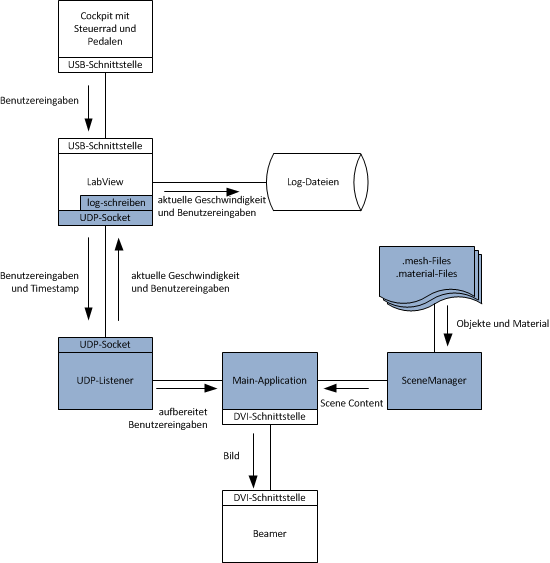
\includegraphics{src/Systembeschreibung.png}
\caption{Systembeschreibung} % Titel der Grafik
\label{Systembeschreibung} % Labelname
\end{figure}


Der Aufbau des Systems für den Fahrsimulator wird anhand der Abbildung \ref{Systembeschreibung} ilustriert. Die blau markierten Komponenten werden im Rahmen dieser Projekt Arbeit entwickelt. Alle übrigen sind bereits vorbestehend. 
Benutzereingaben, die im Cockpit gemacht werden, werden von einem LabView Programm eingelesen. Nun benötigt es einen UDP-Port,  über den verschiedenen Eingaben an das Programm weitergeleitet werden. Es handelt sich hierbei um Werte, die das Drehen des Steuerrades und den Druck auf Gas- oder Bremspedal quantifizieren. Zusätzlich wird der UDP-Port auch für das Empfangen diverser Log-Daten, die von unserem Programm gesendet werden, verwendet. Damit die Empfangenen Daten sauber in ein Log-File geschrieben werden, wird das LabVIEW Programm erweitert. 
Weiter  muss in Programmiersprache C einen UDP-Socket mit entsprechendem UDP-Listener implementieren werden, um die Benutzereingaben zu empfangen. Gleichzeitig wird der UDP-Listener dazu verwendet die Geschwindigkeit des Fahrzeugs sowie Timestamps und weitere Daten an das LabVIEW Programm zurück zu schicken. Damit können die Daten gespeichert und später ausgewertet werden.
\\
Diese Aufteilung durch eine Netzwerkschnittstelle ermöglicht es,  das System, wenn notwendig, zu dezentralisieren. Einfachheitshalber wurde der UDP-Listener erst in einem Video-Beispiel implementier und getestet (Siehe Anhang B). Nachfolgend wird dieser UDP-Listener auch in das Programm des Fahrsimulator transferiert.
Sind die Daten vom UDP-Listener empfangen und aufbereitet, werden sie im Hauptprogramm (Main Application) weiter verwendet. Während die Position des Steuerrades, des Gas und Bremspedales vom UDP-Listener permanent an das Hauptprogramm übertragen werden, wertet dieses die Positionen aus und veranlass die entspechenden Aktionen in der geladenen Szene. 
Die Szene selbst wird von einem Szenen-Manager geladen. Dieser benötig für die zu ladenden Objekte ein Meshfiles und mindestens ein Materialfile. Die Form jedes Objektes in der Szene wird durch ein separates Meshfile definiert. Texturen und Materialien werden durch ein oder mehrere Materialfiles beschrieben. Ein Materialfile kann zur Beschreibung unterschiedlicher Objekte verwendet werden. Die berechnete Szene wird schlussendlich in einem Fenster von Hauptprogramm angezeigt und über eine DVI-Schnittstelle an den Beamer übertragen. Der Beamer projeziert das Bild an die Wand, die sich direkt vor dem Cockpit befindet. 

\subsection{Anforderungen}
\subsubsection{Funktionale Anforderungen}
\begin{itemize}
\item Der Proband kann das Fahrzeug im Fahrsimulator durch manipulation am Steuerrad und der Pedalen im Cockpit steuern.
\item Die aktuelle Geschwindigkeit der Fahzeuges wird dem Probanden angezeigt.
\item Es sollen zwei unterschiedliche Szenen zur verfügung gestellt werden.  Die eine Szene sollte eine Stadt darstellen und die andere Szene eine Landschaft mit Tunnels.
\item Die manipulationen des Benutzers und wichtige Parameter wie z.B. Geschwindigkeit sollen in einer Datei aufgezeichnet werden um diese auszuwerten.
\item Alle ein- und ausgehenden Parameter des System sollen in LabVIEW verfügbar sein um diese auswerten und kontrollieren zu können. 
\end{itemize}

\subsubsection {Nicht Funktionale Anforderungen}
\renewcommand{\labelenumi}{\alph{enumi})}

\begin{itemize}
\item Das System soll robust sein. 
\item Das Starten des Fahrsimulator sollte möglichst einfach gehalten werden. Das Steuer des Fahrzeuges soll möglichst intuitiev sein wie man es sich von einem richtigen Fahrzeug gewöhnt ist. 
\item Der Fahrsimulator soll dem Probanden eine möglichst realistische Fahrsimulation bieten in der sich Strassen und verschiedene Objekte befinden.
\item Die Raktionszeit des Systems soll möglichst klein sein. Die Verzögerung des Systems soll mess-  und kalkulierbar sein.
\item Das System soll möglichst Modular aufgebaut sein um später einfach erweitert werden zu können.
\item Das System soll auf der existierender Hardware funktionieren, soll aber auch noch lauffähig sein wenn Teile des Fahrsimulators ausgetauscht werden. 
\end{itemize}

\section{Vorgehen und Methoden}
Wie bereits in der Systembeschreibung beschrieben, wird der Fahrsimulator in 3 Hauptkomponenten unterteilt. Zum Fahrsimulator gehört ein UDP-Listener, ein Szenen-Manager und das Hauptprogramm. Da die Verbindung zwischen dem Cockpit und dem Fahrsimulator mit einer Netzwerkschnittstelle realisiert wird, ist es möglich die Anbindung an das Cockpit und den Fahrsimulator phisikalisch auf zwei Rechnern zu betreiben. Eine weiter Lösung hätte mit dem Ogre-Framework (Siehe Anhang D?) realisiert werden können. Dieses Framework bietet umfassende Lösungen um Steuerradär und Pedalen, wie sie in userem Cockpit vorhanden sind, anzusteueren.
Da die 3D-Umgebungen mit fortscheitendem Projekt zunimmt, könnte die Rechenleistung der momentan verwendeten Maschiene zu einem späteren Zeitpunkt nicht mehr ausreichen. Die Folgen von ungenügender Leistung können unregelmässige Bewegungen (Lags) in der virtuellen Umgebung sein oder es kann sogar bis zum Absturz des gesamten Programms führen. 
Dieses Problem hat zur Folge, dass
\subsection{UDP-Socket}
permanenter Straem, warum UDP, wie die Variabeln vom Main geholt werden, Packete asynchron -> werte abholen Synchron
\subsection{Virtual Reality}
\subsection{Hautpprogramm}

\lstinputlisting{listings/Karte.java}


%Sequenzdiagramm
%Blockdiagramm


\section{Resultate und Tests}
\subsection{Erreichtes}
\subsection{Zeitliches Verhalten des Systems}
\subsection{Testfälle}
\section{Nächste Schritte}
\subsection{Offene Punkte}
\subsection{Zusätzliche Funktionen}
\subsection{Ausblick auf Bachelor Arbeit 2012}
\section{Nachwort}
\subsection{Danksagung}

\section{Verzeichnisse}
\subsection{Abbildungsverzeichnis}
\listoffigures
\section{Anhang}
\appendix
\section{Aufgabenstellung}
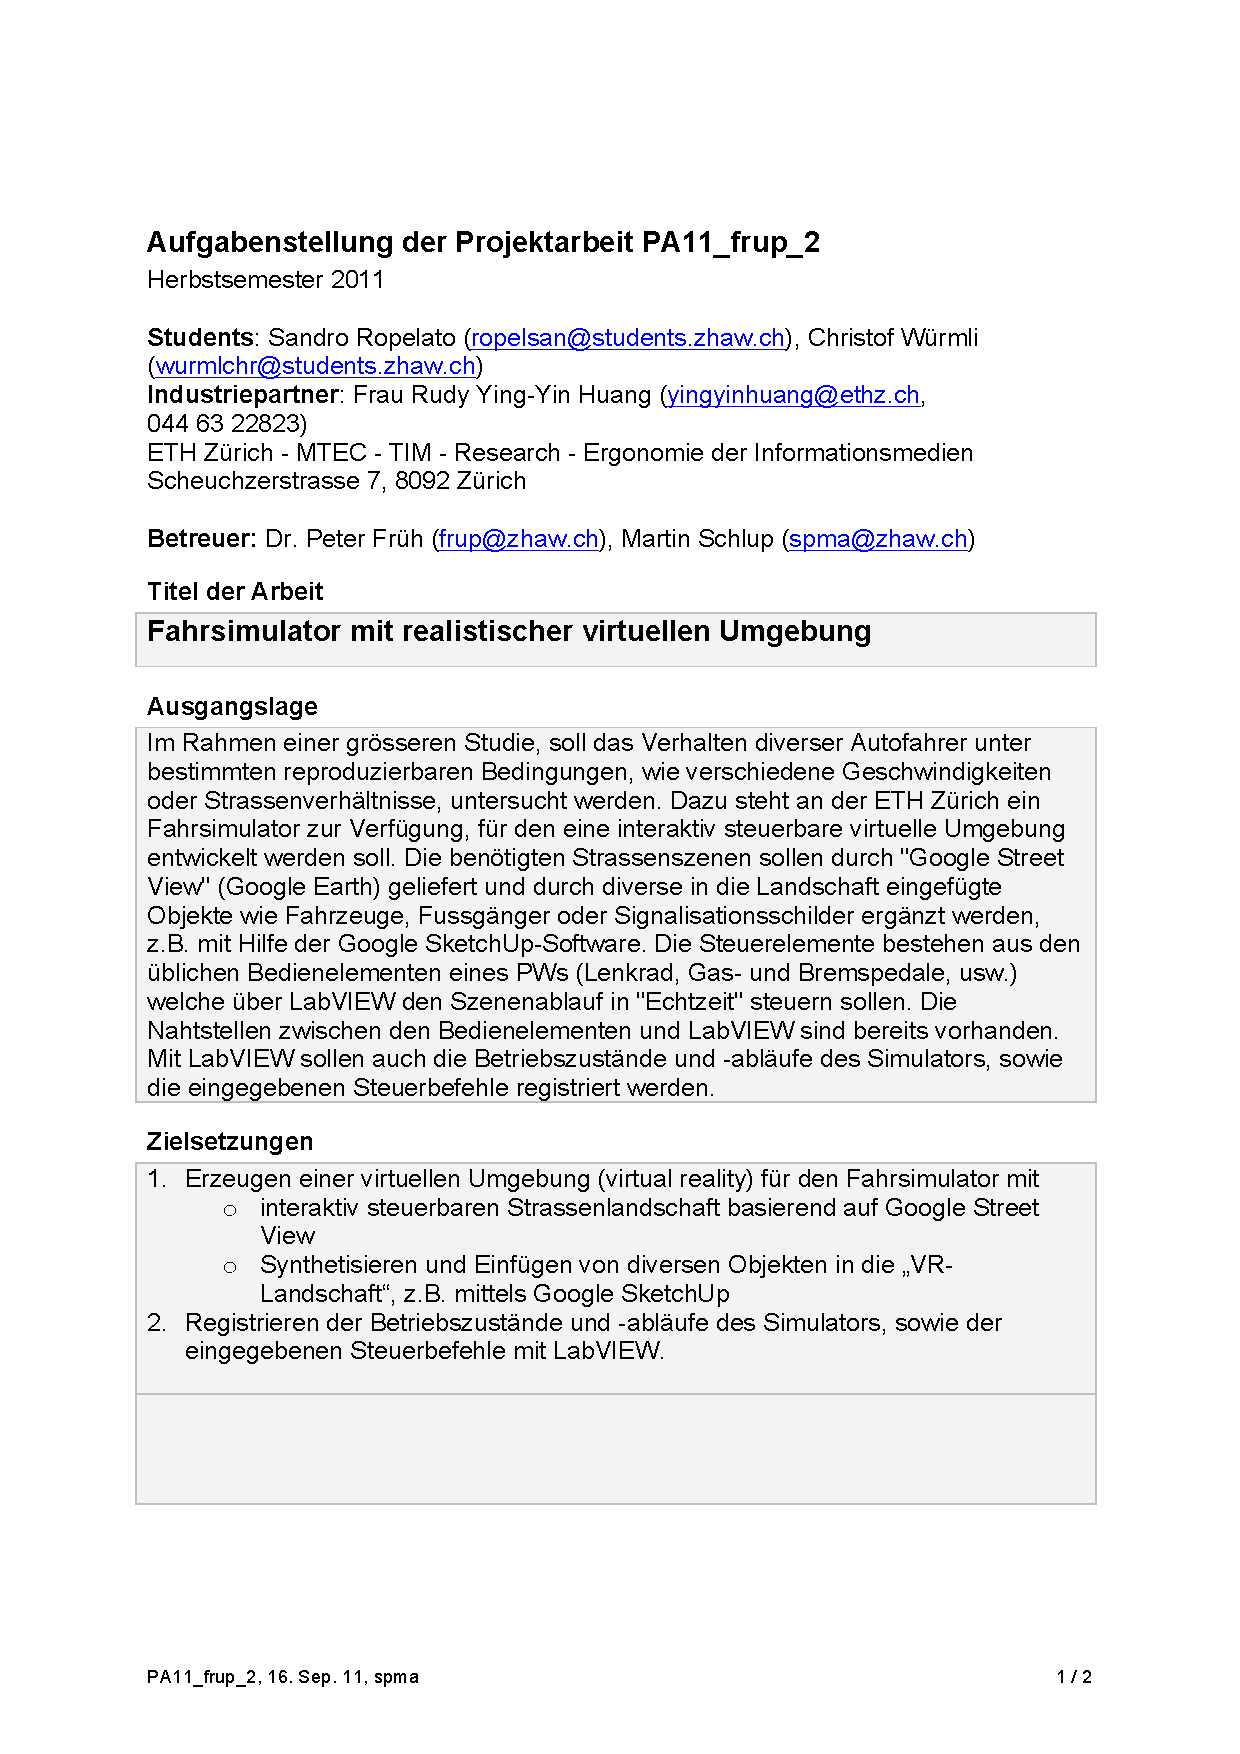
\includepdf[pages=1-2,scale=0.8]{src/PA11_frup_2_Aufgabenstelung.pdf}
\section{Video Player}
\subsection{Ziel}
Um manipulationen im Cockpit zu in unserem Programm zu empfangen zu zu verarbeiten, wird in einem ersten Schritt ein Video-Player realisiert der auf Eingaben des Probanden reagiert. Dies gibt ebenfalls einen ersten Eindruck von einem Fahrverhalten auf dem Simulator. Bei einem Video ist nur die Geschwindigkeit und noch keine Richtung und weiters relevant. Somit wird mit dem Video-Player die Ausgabe sehr reduziert. Ziel im Video-Player ist eine korrekte Übertragung der Eingaben im Cockpit über LabVIEW in das Programm. Das Programm soll die Parameter richtig interpretieren und entsprechende Aktionen veranlassen. Ein weiteres Ziel ist ein korrekte Rückgabe verschiedener Parameter an LabVIEW die von diesem in eine LogDatei geschrieben werden. 
\subsection{Systembeschreibung}

% Bild für Systembeschreibung des Video Players
\begin{figure}[H]
\centering 
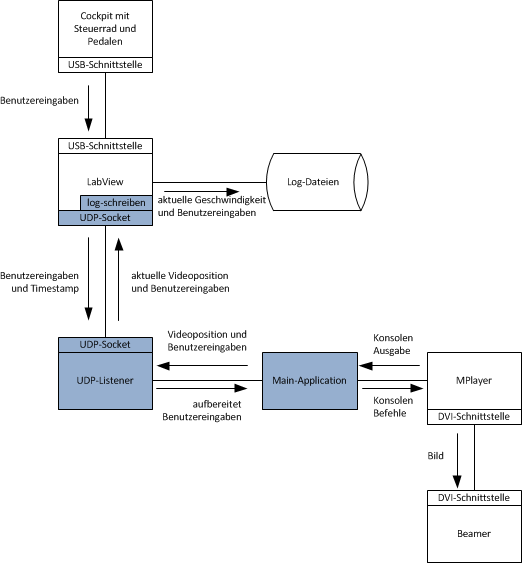
\includegraphics{src/Systembeschreibung_VideoPlayer.png}
\caption{Systembeschreibung Video-Player} % Titel der Grafik
\label{Systembeschreibung Video-Player} % Labelname
\end{figure}
Um einzelne Komponenten des Video-Player wiederverwenden zu können, wird das System möglichst gleich wie das des Fahrsimulators aufgebaut. Dieser Aufbau wird anhand der Abbildung \ref{Systembeschreibung Video-Player} illustriert.  Die blau markierten Komponenten werden im Rahmen des Video-Players entwickelt. Alle überigen sind bereits vorbestehend oder werden installiert und verwendet. 
Die LabVIEW-Komponente in der Abbildung \ref{Systembeschreibung Video-Player} liest bereits die Eingaben die der Proband im Cockpit mach ein. Dieses muss nun so erweitert werden, dass diese über einen UDP-Socket an das Programm übertragen werden. Zusätzlich muss im LabVIEW ein UDP-Port eingerichtet werden, der verwendet werden kann, um UDP-Packete zu empfangen. Dieser wird benötigt um Daten die von unserem Programm gesendet werden in ein Log-File zu schreiben.
Die Parameter werden vom vom UDP-Listener gespeichert und vom Hauptprogramm abgefragt. Aufgrund der Parameter wird dann die Geschwindigkeit des Videos manipuliert. Für das Abspielen des Videos wird der mPlayer verwendet. Die Befehle für den mPlayer können von unserem Programm über die Komandozeile abgesetzt werden. Ausgaben vom mPlayer  werden ebenfalls über die Komandozeile den Standartausgang der Konsole übergeben. 

\subsection{Realisierung}
In einem bestehendem LabVIEW-Programm werden bereits alle Eingaben, die im Cockpit gemacht werden können, eingelesen. Nun muss dieses Programm nur noch mit einem UDP-Port erweitert werden, damit es die Parameter, die unser Video-Player benötigt, senden kann. Diese Daten sind im Video-Player vor allem die betätigung von Gas- und Bremspedal. Diese beiden Pedalen werden in einem Koordinatensystem wie in Abbildung \ref{Koordinatensystem} auf der y-Achse abgebildet. Die positive y-Richtung verifiziert das Gas und die negative y-Richtung das Bremspedal. Die intensität beider Pedalen wird durch 32767 bzw. 32768 ganzzahlige Werte identifiziert. Wenn also keins der beiden Pedalen gedrückt ist, wird dies durch den y-Wert 0 verifiziert. Ein voll gedrücktes Gaspedal entspricht dem y-Wert 32767 und dementsprechend ein voll gedrücktes Bremspedal dem Wert -32768. Der x-Wert im Koordinatensystem verifiziert den Einschlagswinkel des Steuerrades. Ist das Steuerrad in der neutralen Stellung, entspricht dies dem x-Wert null. Wenn das Steuerrad vollständig nach rechts eingeschlagen ist, wird dies durch den positiven x-Wert 32767 identifiziert. Dementsprchend wird ein vollständiger Einschlag nach links durch den negiativen x-Wert -32768 identifiziert. \\

\begin{figure}[H]
\centering 
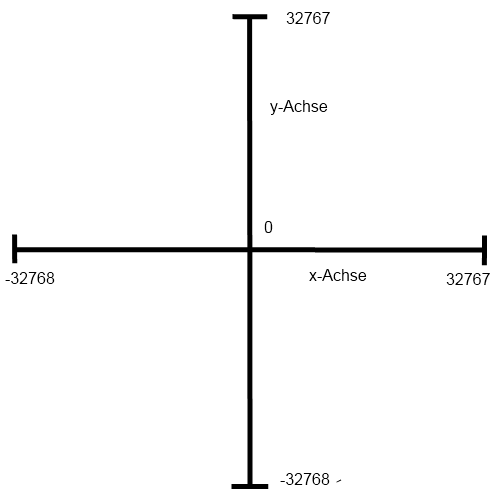
\includegraphics[scale=0.5]{src/koordinatensystem.png}
\caption{Koordinatensystem} % Titel der Grafik
\label{Koordinatensystem} % Labelname
\end{figure}

Diese beiden Werte werden im LabVIEW-Programm in ein UDP-Packet verpackt und über das Netzwerk gesendet. Der UDP-Listener empfängt diese Packete und speichert die x und y-Werte separat ab. Das Hauptprogramm greift auf diese Werte zu, und Steuert damit das Video. 

\section{Das Ogre Framework}
\section{Modelling Tools}

\section{Setup}

\section{Listings}

\section{Detailierter Zeitplan}


\end{document}